\chapter{The Scientific Procedure}

The following activities can be used as a method of introducing students to the scientific method. Rather than just performing the activities, first identify the question or problem with the students, then have them form a hypothesis for each step of the experiment. Students should record observations and data accordingly and use them to draw a conclusion about the activity.

Prepare an activity sheet for each student or have them copy it into their notebooks before performing the activities. Set up stations for the various activities and have students rotate among them in small groups.

After performing several of the experiments, ask students to come up with their own. Ask them to think about problems they face in their daily lives. Encourage interested students to turn their ideas into a science fair project to display for the school or community.

%==================================================================================================%

\section{Biology}


\subsection{Hand Washing}

%\begin{center}
%\includegraphics[width=0.4\textwidth]{./img/source/.jpg}
%\end{center}

\begin{description*}
\item[Materials:]{Soap, water, bottle, basin/bucket, chalk, charcoal, food colour, stopwatch}
\item[Setup:]{Prepare a large amount of soapy water. Grind the chalk and charcoal into separate powders.}\\
\item[Problem:]{How long should we wash our hands?\\

\begin{tabular}{|l|c|c|} \hline
\multirow{2}{*}{\textbf{Material}} & \textbf{Hypothesis} & \multirow{2}{*}{\textbf{Experimental Result}} \\
& \textbf{(Seconds)} & \\ \hline
Chalk powder & & \\ \hline
Charcoal powder & & \\ \hline
Food colour & & \\ \hline
\end{tabular} \\[10pt]
}\\
\item[Hypothesis:]{Predict how much time it will take to completely clean your hands and record in the table.}
\item[Procedure:]{Start a stopwatch and have a student or teacher slowly pour soapy water over a basin while the student washes his or her hands. Stop the clock when the student's hands are completely clean.}
\item[Observations:]{Record the time taken to completely wash your hands in the table.}
\item[Questions:]{}\hfill
\begin{enumerate}
\item Why is it important to wash our hands?
\item When do we need to wash our hands?
\end{enumerate}
\item[Theory:]{Washing our hands with soap and water helps to kill harmful bacteria that can cause us to become sick if allowed into our bodies. It is very important to wash our hands before eating and after using the bathroom.}
\end{description*}

\pagebreak


\subsection{Lung Capacity}

\begin{center}
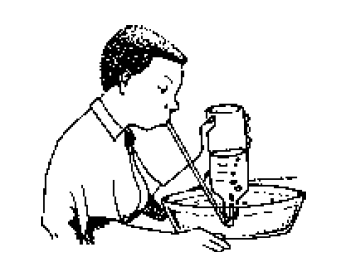
\includegraphics[width=0.4\textwidth]{./img/source/lung-capacity.png}
\end{center}

\begin{description*}
\item[Materials:]{1.5 L bottle, basin, water, plastic tubes/straws, soap, marker, ruler}
\item[Setup:]{Make a scale on the bottle using a marker and ruler (e.g. 100 mL increments). Prepare a soap solution for washing the tubes/straws}\\
\item[Problem:]{How much air can your lungs hold?\\

\begin{tabular}{|l|c|c|} \hline
\multirow{2}{*}{\textbf{Breath}} & \textbf{Hypothesis} & \multirow{2}{*}{\textbf{Experimental Result}} \\
& \textbf{(Volume of air in mL)} & \\ \hline
Normal breath & & \\ \hline
Full breath & & \\ \hline
After holding breath for 10 seconds & & \\ \hline
\end{tabular} \\[10pt]
}
\item[Hypothesis:]{Record the volume of air that you think the lungs can hold for each case in the table.}
\item[Procedure:]{Fill a basin with water. Fill a 1.5 L bottle with water and invert it in the basin so that the mouth of the bottle is underneath the water. Place one end of the tube/straw inside the bottle under water. For each breath, blow into the tube to displace the water.}
\item[Observations:]{Note the reading on the scale before and after blowing into the tube and record the \emph{difference} to give the amount of water displaced.}
\item[Questions:]{}\hfill
\begin{enumerate}
\item Which breath produces the largest amount of air? Which give the smallest amount?
\item How long can you hold your breath?
	\begin{enumerate}
	\item[] Hypothesis: I can hold my breath for \_\_\_\_\_\_\_ seconds.
	\item[] Experimental Result: I can hold my breath for \_\_\_\_\_\_\_ seconds.
	\end{enumerate}
\end{enumerate}
\item[Theory:]{When we breath in air, our bodies use the oxygen and produce carbon dioxide in a process called \emph{respiration}. Oxygen is transported in our blood throughout our bodies. When we hold our breath, oxygen is not circulated throughout our bodies and we begin to feel lightheaded.}
\end{description*}

\pagebreak


%==================================================================================================%

\section{Chemistry}


\subsection{Acids and Bases}

\begin{center}
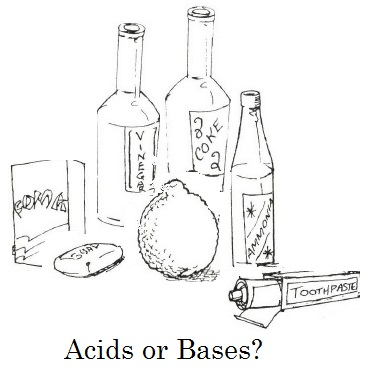
\includegraphics[width=0.4\textwidth]{./img/source/acids-bases-sci-meth.jpg}
\end{center}

\begin{description*}
\item[Materials:]{Bottles, bottle caps, water, vinegar, lemons, baking soda, soda, soap, antacid tablets, rosella leaves, straws/syringes}
\item[Setup:]{Prepare solutions for each of the items above in separate bottles. Prepare indicator by placing rosella leaves in hot water.}\\
\item[Problem:]{What differences can we observe among acids and bases?\\

\begin{tabular}{|l|c|c|} \hline
\multirow{2}{*}{\textbf{Solutions}} & \textbf{Hypothesis} & \multirow{2}{*}{\textbf{Experimental Result}} \\
& \textbf{(Which is different?)} & \\ \hline
Vinegar, lemon, baking soda & & \\ \hline
Vinegar, baking soda, soap & & \\ \hline
Baking soda, antacid, soda & & \\ \hline
Soda, soap, vinegar & & \\ \hline
\end{tabular} \\[10pt]
}
\item[Hypothesis:]{For each set of solutions, which one will reveal a colour different from the others? Record your predictions in the table.}
\item[Procedure:]{Place small amounts of 3 different solutions in separate bottle caps according to the table. Add a few drops of rosella indicator to each.}
\item[Observations:]{Record observations of colour change under \emph{Experimental Result} in the table.}
\item[Questions:]{\hfill
\begin{enumerate}
\item Which solutions have similar properties?
\item Which solutions are acids? What colour do they show?
\item Which solutions are bases? What colour do they show?
\end{enumerate}
}
\item[Theory:]{Coloured leaves such as rosella act as indicators for identifying acids and bases. Adding rosella indicator reveals a red colour for acids and a blue colour for bases. Students do not need to understand the differences between acids and bases in order to observe their different behaviours. Locally available examples of acids include sour milk, citrus fruits and soda. Local bases include ammonia, toothpaste and detergent.}
\end{description*}

\pagebreak

\subsection{Mixing Acids and Bases}

\begin{center}
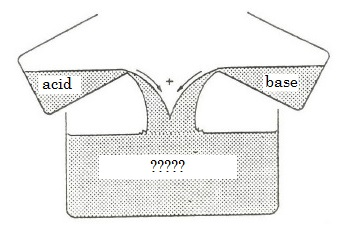
\includegraphics[width=0.6\textwidth]{./img/source/mixing-acid-base.jpg}
\end{center}

\begin{description*}
\item[Problem:]{What happens when acids and bases are mixed together?\\

\begin{tabular}{|l|c|c|} \hline
\multirow{2}{*}{\textbf{Solutions to Mix}} & \textbf{Hypothesis} & \multirow{2}{*}{\textbf{Experimental Result}} \\
& \textbf{(What colour?)} & \\ \hline
Mix vinegar and lemon & & \\ \hline
Mix baking soda and soap & & \\ \hline
Mix vinegar and baking soda & & \\ \hline
\end{tabular}\\[10pt]
}
\item[Hypothesis:]{Predict any colour changes or observations when pairs of solutions are mixed together. Record in the table.}
\item[Procedure:]{Mix small amounts of solutions together according to the table.}
\item[Observations:]{Record observations (colour changes, etc.) in the table.}
\item[Questions:]{\hfill
\begin{enumerate}
\item What happens when an acid is mixed with an acid?
\item What happens when a base is mixed with a base?
\item What happens when an acid is mixed with a base?
\end{enumerate}
}
\item[Theory:]{Mixing acids with acids and bases with bases may cause the colour of the solution to turn darker or lighter depending on the solutions used. Mixing an acid with a base should reveal a colourless solution and produce carbon dioxide gas. You may need to vary the amounts of acid and base to get a colourless solution depending on their concentrations.}
\end{description*}

\pagebreak


%\subsection{Separation of Mixtures}
%
%%\begin{center}
%%\includegraphics[width=0.4\textwidth]{./img/source/.jpg}
%%\end{center}
%
%\begin{description*}
%\item[Materials:]{Bottles, salt, water, rice, beans, steel wool, paper, cloth, oil, wire mesh (sieve), sand, maize seeds, magnet}
%\item[Setup:]{}\\
%\item[Problem:]{\\
%
%\begin{tabular}{|l|c|c|} \hline
%\multirow{2}{*}{\textbf{Mixture}} & \textbf{Hypothesis} & \multirow{2}{*}{\textbf{Experimental Result}} \\
%& \textbf{(Filtration, Decantation, Distillation, Chromatography, Magnet)} & \\ \hline
%Water and sand& & \\ \hline
%& & \\ \hline
%\end{tabular} \\[10pt]
%}\\
%\item[Hypothesis:]{}
%\item[Procedure:]{}
%\item[Observations:]{}
%\item[Questions:]{}\hfill
%\begin{enumerate}
%\item 
%\end{enumerate}
%\item[Theory:]{}
%\end{description*}

%==================================================================================================%

\section{Physics}


\subsection{Complete the Circuit}

\begin{center}
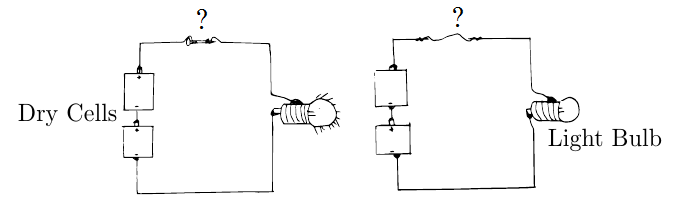
\includegraphics[width=0.8\textwidth]{./img/conductors-insulators-sci-meth.png}
\end{center}

\begin{description*}
\item[Materials:]{Dry cell, speaker wire, bulb/ammeter, cardboard, various objects, e.g. rubber band, nail, paper, aluminum foil, toothpick, pen, scissors, bottle cap, coin, balloon, chalk}
\item[Setup:]{Connect a dry cell and bulb in series using speaker wire and attach to a sheet of cardboard. Leave two wires free and pin to the cardboard to act as a switch.}
\item[Problem:]{Which objects will light a bulb?\\

\begin{tabular}{|l|c|c|} \hline
\multirow{2}{*}{\textbf{Object}} & \textbf{Hypothesis} & \multirow{2}{*}{\textbf{Experimental Result}} \\
& \textbf{(Light or No Light)} & \\ \hline
Copper wire & & \\ \hline
Pen & & \\ \hline
Aluminum foil& & \\ \hline
Paper& & \\ \hline
Nail& & \\ \hline
Toothpick& & \\ \hline
Bottle cap& & \\ \hline
Balloon& & \\ \hline
Chalk& & \\ \hline
Scissors (blade)& & \\ \hline
Scissors (handle)& & \\ \hline
\end{tabular}\\[10pt]
}
\item[Hypothesis:]{Predict which materials will cause the bulb to light when placed across the switch. Record predictions in the table.}
\item[Procedure:]{Test each object by placing it across the free wires to close the circuit.}
\item[Observations:]{Record the result for each item in the table.}
\item[Questions:]{}\hfill 
\begin{enumerate}
\item Which materials caused the bulb to light?
\item These objects are made from what kind or materials?
\item What other objects in the room can you find to test? Will they light the bulb?
\end{enumerate}
\item[Theory:]{\emph{Conductors} are materials which easily allow electrons to flow through them. \emph{Insulators} are materials which do not easily allow the the flow of electrons. Examples of good conductors are most metals, water and the human body. Examples of good insulators are rubber, wood and plastic.}
\end{description*}

\pagebreak


\subsection{Density Tower}

\begin{center}
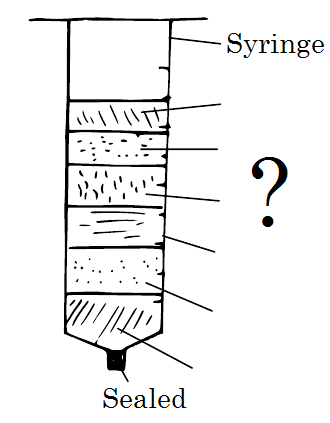
\includegraphics[width=0.3\textwidth]{./img/density-tower-sci-meth.png}
\end{center}

\begin{description*}
\item[Materials:]{Syringes, bottles, water, cooking oil, kerosene, spirit, honey, glycerine, tape, scissors}
\item[Setup:]{Prepare a test tube rack by cutting a bottle and filling it with dirt. Remove the plungers from the syringes and seal them with tape, super glue, or by melting to opening closed.}\\
\item[Problem:]{Which liquids are more dense than others?\\

\begin{tabular}{|l|c|c|} \hline
\multirow{2}{*}{\textbf{Liquid}} & \textbf{Hypothesis} & \multirow{2}{*}{\textbf{Experimental Result}} \\
& \textbf{(Position, 1 = bottom)} & \\ \hline
Water & & \\ \hline
Cooking oil & & \\ \hline
Kerosene & & \\ \hline
Spirit & & \\ \hline
Honey & & \\ \hline
Glycerine & & \\ \hline
\end{tabular} \\[10pt]
}\\
\item[Hypothesis:]{Predict the order in which the liquids will settle from the bottom of the syringe. Assign 1 to the bottom liquid, 2 to the one above it, and so on.}
\item[Procedure:]{Pour a small amount of each liquid into a syringe, observing after each addition.}
\item[Observations:]{After adding all liquids, record the order in which they rest, starting with 1 at the bottom.}
\item[Questions:]{}\hfill
\begin{enumerate}
\item Which liquid finished at the bottom?
\item Which liquid finished at the top?
\item Which liquid has the greatest density?
\item Which liquid has the lowest density?
\item What happens if you place a small object (e.g. paper clip, eraser, paper) in the tower? 
\end{enumerate}
\item[Theory:]{\emph{Density} is a property of different materials and liquids. It is a ratio of its mass to its volume. Dense liquids sink to the bottom, while less dense liquids rise to the top. A small object placed in the tower will settle in the liquid which is nearest its own density.}
\end{description*}

\pagebreak


\subsection{Sinkers and Floaters}

%\begin{center}
%\includegraphics[width=0.4\textwidth]{./img/source/.jpg}
%\end{center}

\begin{description*}
\item[Materials:]{Basin of water, various objects, e.g. nail, paper clip, paper, aluminum foil, soda cap, matchbox, pen cap, toothpick, balloons, flour}
%\item[Setup:]{}\\
\item[Problem:]{Which objects sink or float when placed in water?\\

\begin{tabular}{|l|c|c|} \hline
\multirow{2}{*}{\textbf{Object}} & \textbf{Hypothesis} & \multirow{2}{*}{\textbf{Experimental Result}} \\
& \textbf{(Sink or Float)} & \\ \hline
Nail& & \\ \hline
Paper clip& & \\ \hline
Pen cap& & \\ \hline
Soda cap (dropped)& & \\ \hline
Soda cap (placed carefully)& & \\ \hline
Toothpick & & \\ \hline
Paper& & \\ \hline
Aluminum foil& & \\ \hline
Matchbox& & \\ \hline
Balloon (empty)& & \\ \hline
Balloon (filled with flour)& & \\ \hline
Balloon (filled with water)& & \\ \hline
Balloon (filled with air)& & \\ \hline
\end{tabular} \\[10pt]
}\\
\item[Hypothesis:]{Predict whether each object will sink or float when placed in the basin of water. Record in the table.}
\item[Procedure:]{Place each object in the water. First place them very carefully, then drop them in.}
\item[Observations:]{Record the results in the table.}
\item[Questions:]{}\hfill
\begin{enumerate}
\item What factors affect whether an object sinks or floats?
\item How do large objects such as boats float?
\end{enumerate}
\item[Theory:]{\emph{Flotation} depends on several things. A bottle cap placed carefully on the surface of the water will float, but when pushed under, will sink. A sheet of aluminum foil will float while a sheet of the same size which is folded several times will sink. A balloon filled with flour sinks, one filled with water just floats, and one filled with air floats above the surface.\\

If an object's \emph{total density} is greater than that of water, it sinks, but if less than water, it floats. Air has a density less than water, so when air is trapped in objects such as bottle caps or balloons, they float because their total density is less than water. When air is removed (folded aluminum foil) or replaced by water (bottle cap), the total density of the object is just the density of the material. A matchbox pushed under water rises back to the surface because its density is less than that of water.\\

Boats are able to float despite being built from dense materials because of the large volume of water they displace and the large amount of air inside the boat. A boat with a larger surface area displaces a larger volume of water and thus can carry a larger load before sinking.\\

Follow up this activity with the \emph{Raft Rally} science competition.}
\end{description*}

\pagebreak


\subsection{Mixing Colours}

%\begin{center}
%\includegraphics[width=0.4\textwidth]{./img/source/.jpg}
%\end{center}

\begin{description*}
\item[Materials:]{Various food colours, syringes, bottle, scissors, tape, paper}
\item[Setup:]{Prepare a test tube rack by cutting a bottle and filling it with dirt. Remove the plungers from the syringes and seal them with tape, super glue, or by melting to opening closed.}\\
\item[Problem:]{What happens when we mix different colours?\\

\begin{tabular}{|l|c|c|} \hline
\multirow{2}{*}{\textbf{Colours to Mix}} & \textbf{Hypothesis} & \multirow{2}{*}{\textbf{Experimental Result}} \\
& \textbf{(What colour?)} & \\ \hline
Red and green & & \\ \hline
Yellow and blue & & \\ \hline
Red and yellow & & \\ \hline
All colours & & \\ \hline
\end{tabular} \\[10pt]
}\\
\item[Hypothesis:]{Predict which colour will result when the two colours given are mixed together. Record it in the table.}
\item[Procedure:]{Use syringes to remove small amounts of each colour and place on a sheet of paper. Be sure to lay down plenty of paper so that the colours do not bleed through onto the table!}
\item[Observations:]{Record the resulting colour mixture in the table.}
\item[Questions:]{}\hfill
\begin{enumerate}
\item How can you make orange from other colours?
\item What colour do you get by mixing all of the colours together?
\item What are some uses of coloured dyes?
\end{enumerate}
\item[Theory:]{Red, green and blue are \emph{primary colours} of light. Other colours are made by different combinations of these primary colours. Coloured dyes are used for many applications, including clothes, paper and printing pictures.}
\end{description*}



